% this file is called up by thesis.tex
% content in this file will be fed into the main document
\chapter{Código/Manuales/Publicaciones}
% top level followed by section, subsection

\section{Validación del intrumento de medición por parte de los expertos}

\begin{figure}[H]
	\centering
	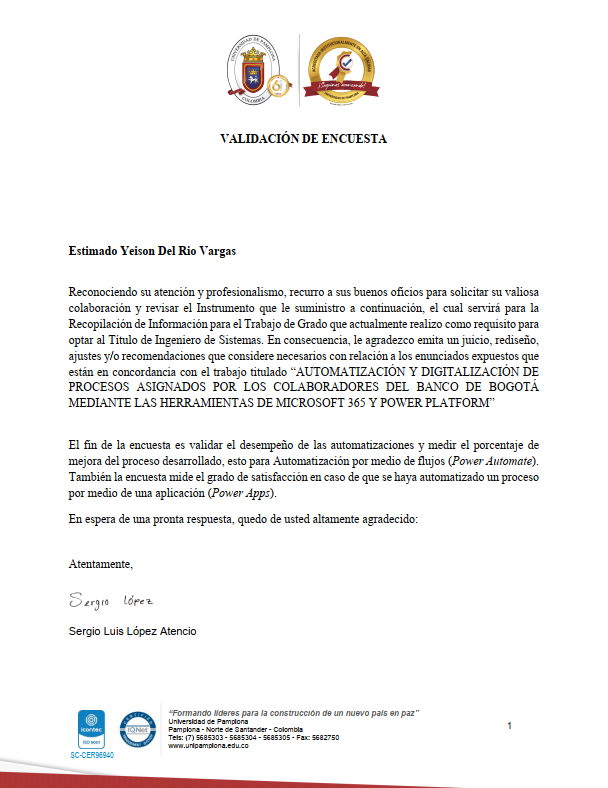
\includegraphics[scale=0.4]{Capitulo6/1}
	\label{anexo1}
	\caption{Anexo 1}
\end{figure}

\begin{figure}[H]
	\centering
	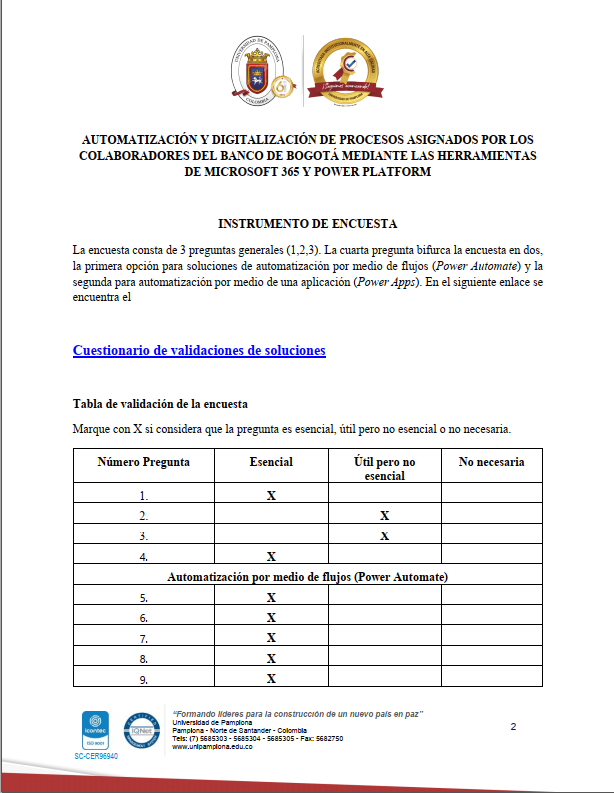
\includegraphics[scale=0.4]{Capitulo6/2}
	\label{anexo2}
	\caption{Anexo 2}
\end{figure}

\begin{figure}[H]
	\centering
	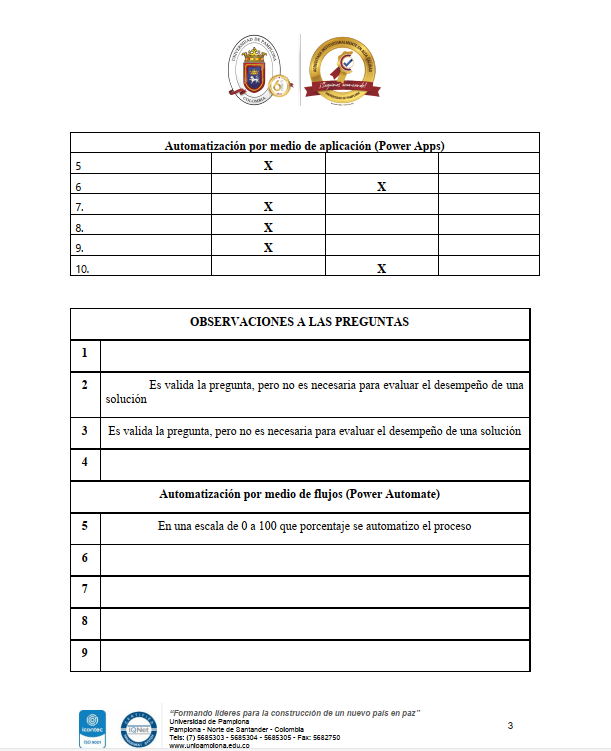
\includegraphics[scale=0.4]{Capitulo6/3}
	\label{anexo3}
	\caption{Anexo 3}
\end{figure}

\begin{figure}[H]
	\centering
	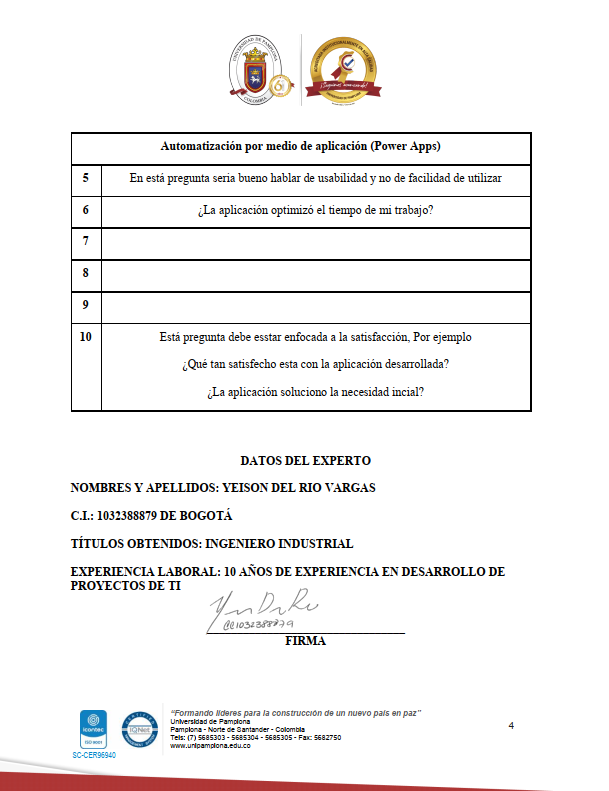
\includegraphics[scale=0.4]{Capitulo6/4}
	\label{anexo4}
	\caption{Anexo 5}
\end{figure}

\begin{figure}[H]
	\centering
	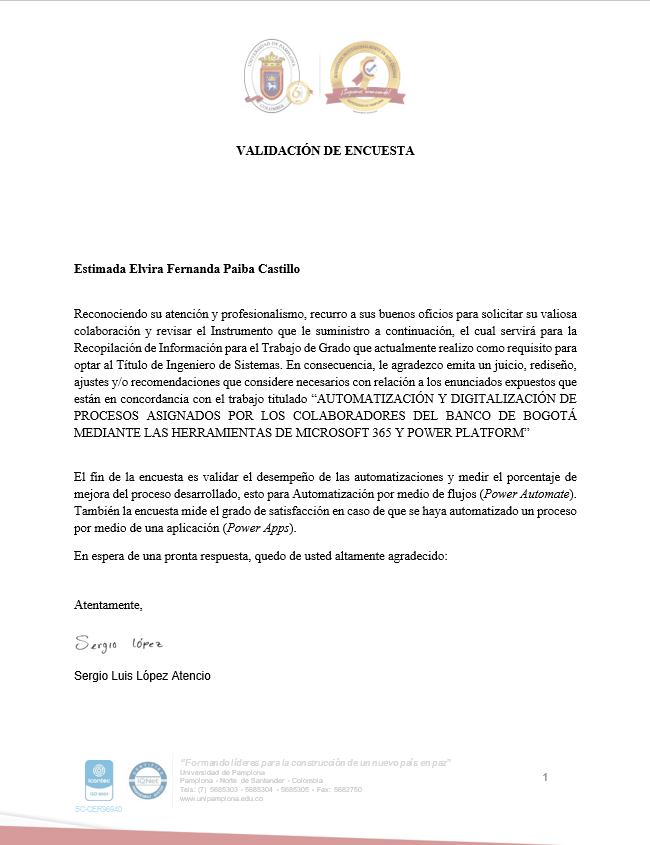
\includegraphics[scale=0.4]{Capitulo6/5}
	\label{anexo5}
	\caption{Anexo 5}
\end{figure}

\begin{figure}[H]
	\centering
	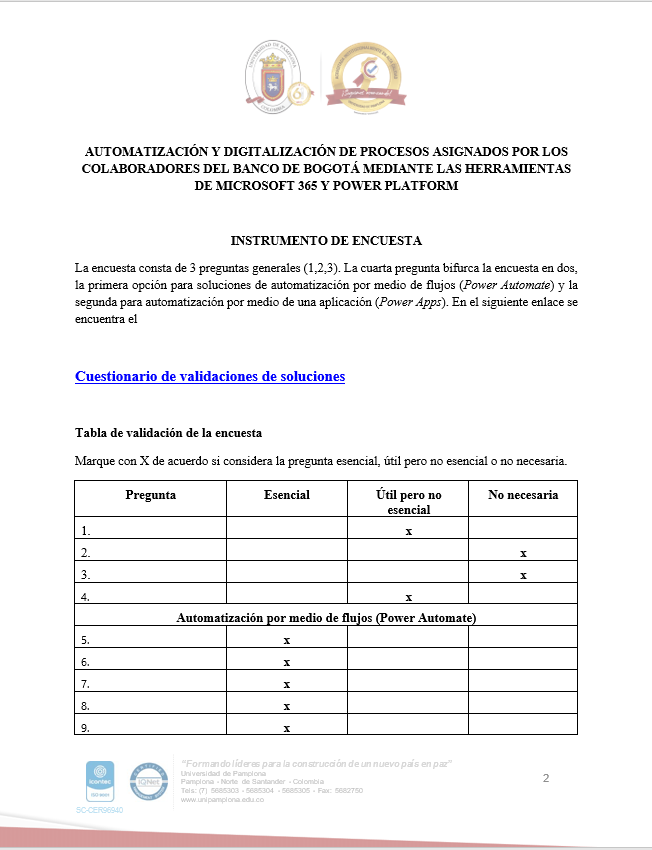
\includegraphics[scale=0.4]{Capitulo6/6}
	\label{anexo6}
	\caption{Anexo 6}
\end{figure}

\begin{figure}[H]
	\centering
	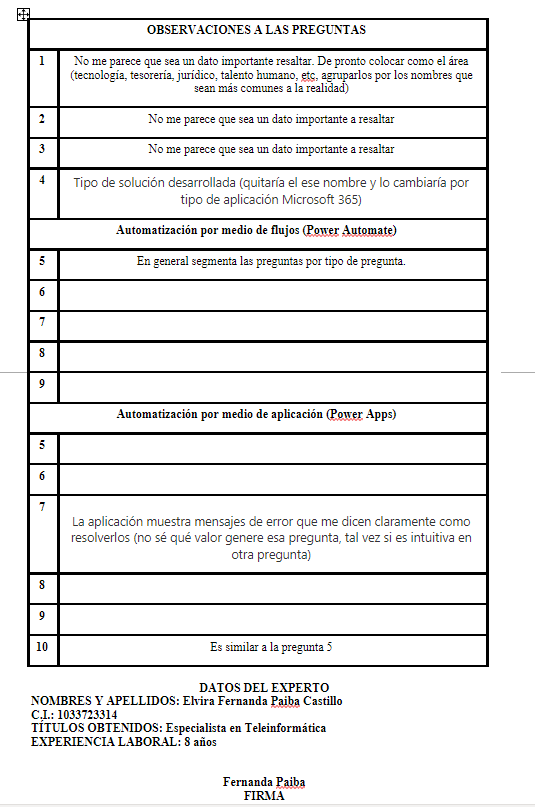
\includegraphics[scale=0.4]{Capitulo6/7}
	\label{anexo7}
	\caption{Anexo 7}
\end{figure}

\begin{figure}[H]
	\centering
	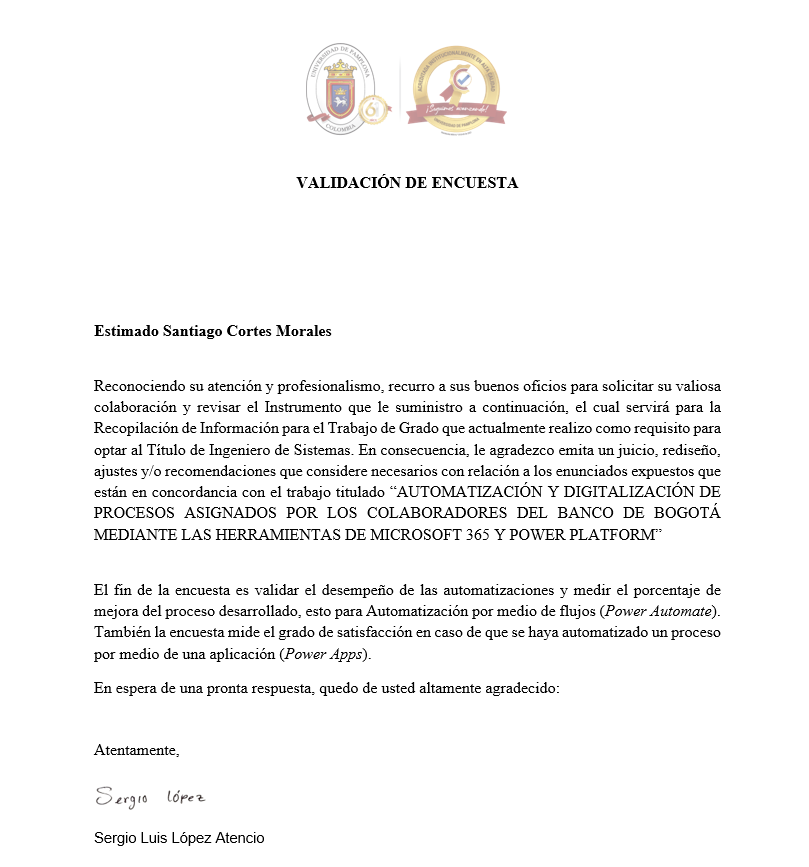
\includegraphics[scale=0.4]{Capitulo6/8}
	\label{anexo8}
	\caption{Anexo 8}
\end{figure}

\begin{figure}[H]
	\centering
	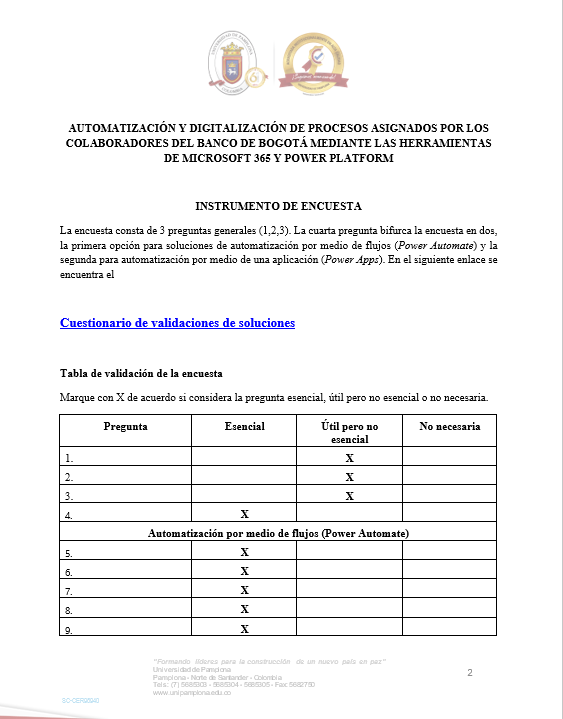
\includegraphics[scale=0.4]{Capitulo6/9}
	\label{anexo9}
	\caption{Anexo 9}
\end{figure}

\begin{figure}[H]
	\centering
	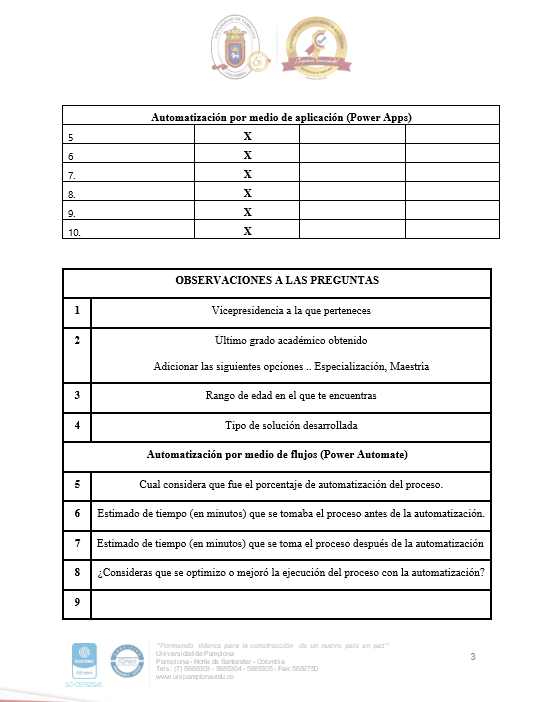
\includegraphics[scale=0.4]{Capitulo6/10}
	\label{anexo10}
	\caption{Anexo 10}
\end{figure}

\begin{figure}[H]
	\centering
	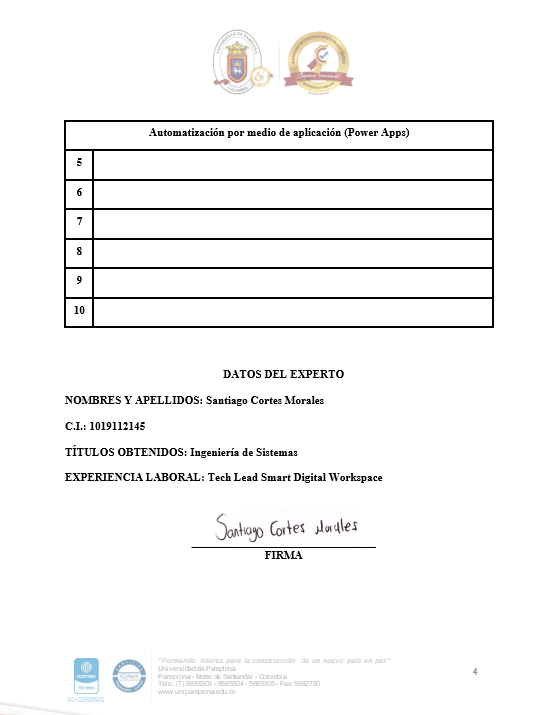
\includegraphics[scale=0.4]{Capitulo6/11}
	\label{anexo11}
	\caption{Anexo 11}
\end{figure}

